\documentclass{tufte-handout}

\title{A program to convert any number into Binary}

\author[EF Academy]{Neel Ramani}

%\geometry{showframe} % display margins for debugging page layout

\usepackage{graphicx} % allow embedded images
  \setkeys{Gin}{width=\linewidth,totalheight=\textheight,keepaspectratio}
  \graphicspath{{graphics/}} % set of paths to search for images
\usepackage{amsmath}  % extended mathematics
\usepackage{booktabs} % book-quality tables
\usepackage{units}    % non-stacked fractions and better unit spacing
\usepackage{multicol} % multiple column layout facilities
\usepackage{lipsum}   % filler text
\usepackage{fancyvrb} % extended verbatim environments
  \fvset{fontsize=\normalsize}% default font size for fancy-verbatim environments
  
  
  
  \usepackage[T1]{fontenc} % Use 8-bit encoding that has 256 glyphs
\usepackage{fourier} % Use the Adobe Utopia font for the document - comment this line to return to the LaTeX default
\usepackage[english]{babel} % English language/hyphenation
\usepackage{amsmath,amsfonts,amsthm} % Math packages
\usepackage{mathtools}% http://ctan.org/pkg/mathtools
\usepackage{etoolbox}% http://ctan.org/pkg/etoolbox
\usepackage{lipsum} % Used for inserting dummy 'Lorem ipsum' text into the template
\usepackage{units}% To use \nicefrac
\usepackage{cancel}% To use \cancel
%\usepackage{physymb}%To use r
\usepackage{sectsty} % Allows customizing section commands
\usepackage[dvipsnames]{xcolor}
\usepackage{pgf,tikz}%To draw 
\usepackage{pgfplots}%To draw 
\usetikzlibrary{shapes,arrows}%To draw 
\usetikzlibrary{patterns,fadings}
 \usetikzlibrary{decorations.pathreplacing}%To draw curly braces 
 \usetikzlibrary{snakes}%To draw 
 \usetikzlibrary{spy}%To do zoom-in
 \usepackage{setspace}%Set margins and such
 %\usepackage{3dplot}%To draw in 3D
\usepackage{framed}%To get shade behind text


\definecolor{shadecolor}{rgb}{0.9,0.9,0.9}%setting shade color
\allsectionsfont{\centering \normalfont\scshape} % Make all sections centered, the default font and small caps
  
  

  
  

% Standardize command font styles and environments
\newcommand{\doccmd}[1]{\texttt{\textbackslash#1}}% command name -- adds backslash automatically
\newcommand{\docopt}[1]{\ensuremath{\langle}\textrm{\textit{#1}}\ensuremath{\rangle}}% optional command argument
\newcommand{\docarg}[1]{\textrm{\textit{#1}}}% (required) command argument
\newcommand{\docenv}[1]{\textsf{#1}}% environment name
\newcommand{\docpkg}[1]{\texttt{#1}}% package name
\newcommand{\doccls}[1]{\texttt{#1}}% document class name
\newcommand{\docclsopt}[1]{\texttt{#1}}% document class option name
\newenvironment{docspec}{\begin{quote}\noindent}{\end{quote}}% command specification environment

\begin{document}

\maketitle% this prints the handout title, author, and date
\begin{marginfigure}%
  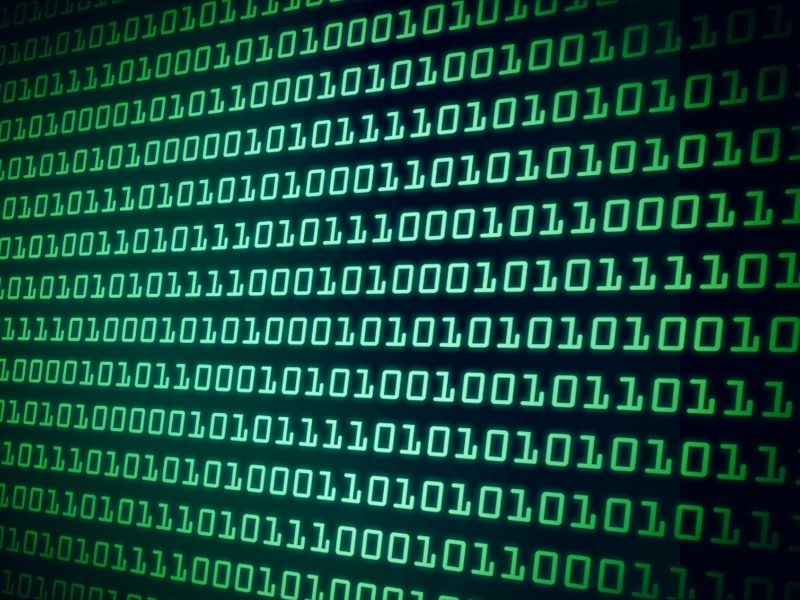
\includegraphics[width=\linewidth]{binary.jpeg}
  \caption{This is the picture showing some binary process.}
  \label{fig:marginfig}
\end{marginfigure}
\begin{abstract}
\noindent
In this report I will present my code which will convert the number input to binary.
\end{abstract}

\normalsize

%this generates 1cm of vertical space
\vspace{1cm}
\section{Software}

This is what you will need for the following code or Program to work

\begin{shaded}
\begin{verbatim}
Python 2.7.10 Downloaded and installed
\end{verbatim}
\end{shaded}

\vspace{1cm}

\section{Python Code}

\marginnote[40pt]{Enter a number you want to convert into binary and hit enter.You will be asked to again input the same number. Then the following code will convert the number into binary }

\begin{framed}
\begin{verbatim}

while True:
    c=int(input("Enter a number to conver into binary   "))
    a=int(input("Enter the number again     "))
    b=2
    e=0
    ans=""

    while c>(b**e):
        m=a%(b**(e+1))
        n=m/(b**e)
        ans=str(n)+ans
        a=a-m
        e=e+1

    print"The binary number is "+ ans

\end{verbatim}
\end{framed}

\marginnote[40pt]{The code will output the following line but with the binary form of the number you put in and after the binary number is displayed it will start the process from beginning hence asking you again to put a number to be converted to binary}

\begin{shaded}
\begin{verbatim}
The binary number is  _________
\end{verbatim}
\end{shaded}

\bibliography{sample-handout}
\bibliographystyle{plainnat}



\end{document}
